\documentclass[12pt]{article}
\usepackage{Sweave}
\usepackage{myVignette}
\usepackage[authoryear,round]{natbib}
\bibliographystyle{plainnat}
\DefineVerbatimEnvironment{Sinput}{Verbatim}
{formatcom={\vspace{-2.5ex}},fontshape=sl,
  fontfamily=courier,fontseries=b, fontsize=\scriptsize}
\DefineVerbatimEnvironment{Soutput}{Verbatim}
{formatcom={\vspace{-2.5ex}},fontfamily=courier,fontseries=b,%
  fontsize=\scriptsize}
%%\VignetteIndexEntry{Sparse matrix representations of linear mixed models}
%%\VignetteDepends{Matrix}
%%\VignetteDepends{lme4}
\begin{document}

\setkeys{Gin}{width=\textwidth}
\title{Sparse Matrix Representations of Linear Mixed Models}
\author{Douglas Bates\\Department of Statistics\\University of
  Wisconsin -- Madison\\\email{Bates@wisc.edu}}
\date{June 18, 2004}
\maketitle
\begin{abstract}
  We describe a representation of linear mixed-effects models using a
  sparse semidefinite matrix.  This representation provides for efficient
  evaluation of the profiled log-likelihood or profiled restricted
  log-likelihood of the model, given the relative precision parameters
  for the random effects.  The evaluation is based upon the
  $\bL\bD\bL\trans$ form of the Cholesky decomposition of the
  augmented sparse representation.  Additionally, we can use
  information from this representation to evaluate ECME updates and
  the gradient of the criterion being optimized.
  
  The sparse matrix methods that we employ have both a symbolic phase,
  in which the number and the positions of nonzero elements in the
  result are determined, and a numeric phase, in which the actual
  numeric values are determined.  The symbolic phase need only be done
  once and it can be accomplished knowing only the grouping factors
  with which the random effects are associated. An important part of
  the symbolic phase is determination of a fill-minimizing permutation
  of the rows and columns of the sparse semidefinite matrix.  This
  matrix has a special structure in the linear mixed-effects problem
  and we provide a new fill-minimizing algorithm tuned to this
  structure.

\end{abstract}

\section{Introduction}
\label{sec:Intro}

Mixed-effects models, also called multilevel models, panel data
models, and frailty models, are widely used in many areas of
statistical applications \citep{pinh:bate:2000}.  The basic form of
the model, the linear mixed model, also serves as an approximation in
iterative estimation of the parameters in more general forms such as
the generalized linear mixed model (GLMM) and the nonlinear mixed
model (NMM).

In \S\ref{sec:LinearMixed} we define a general form of a linear mixed
model using grouping factors and model matrices associated
with these grouping factors.  This form, which can be used for multiple
levels of random effects in either nested or crossed configurations,
can be represented and manipulated using a sparse, symmetric,
semidefinite matrix and several dense matrices.  We show that a
profiled log-likelihood can be evaluated from the solution to a
penalized least squares problem and that this solution can be obtained
from the Cholesky decomposition of an augmented form of the sparse,
symmetric matrix.

Many implementations of the Cholesky decomposition of sparse,
symmetric, semidefinite matrices have both a symbolic phase, in which
the number and the positions of nonzero elements in the result are determined,
and a numeric phase, in which the actual numeric values are
determined.  In \S\ref{sec:Symbolic} we show that the symbolic
analysis for the matrices we consider need only be done once and can
be accomplished knowing only the grouping factors.  An important part
of the symbolic phase is determination of a fill-reducing permutation
of the rows and columns of the symmetric matrix.  We show that by
suitably ordering the grouping factors and by restricting ourselves to
permutations that correspond to reorderings of the levels within the
grouping factors we can determine effective fill-reducing orderings.

Finally, in \S\ref{sec:Generalizations} we show how these methods can be
used to implement general penalized least squares approaches to models
such as the GLMM and the NMM and then to implement more accurate
approximations to the marginal likelihood using Laplacian integration
or adaptive Gauss-Hermite integration.

\section{Linear mixed models}
\label{sec:LinearMixed}

We describe the form of the linear mixed-effects model that we will
consider and restate some of the formulas from \citet{bate:debr:2004}
using the LDL form of the Cholesky decomposition of a sparse,
semidefinite matrix.

\subsection{Form of the model}
\label{ssec:ModelForm}

We consider linear mixed-effects models that can be written as
\begin{equation}
  \label{eq:lmeGeneral}
  \by=\bX\bbeta+\bZ\bb+\beps\quad
  \beps\sim\mathcal{N}(\bzer,\sigma^2\bI),
  \bb\sim\mathcal{N}(\bzer,\sigma^2\bOmega^{-1}),
  \beps\perp\bb
\end{equation}
where $\by$ is the $n$-dimensional response vector, $\bX$ is an
$n\times p$ model matrix for the $p$-dimensional fixed-effects vector
$\bbeta$, $\bZ$ is the $n\times q$ model matrix for the
$q$-dimensional random-effects vector $\bb$ that has a Gaussian
distribution with mean $\bzer$ and relative precision matrix $\bOmega$
(i.e., $\bOmega$ is the precision of $\bb$ relative to the precision
of $\beps$), and $\beps$ is the random noise assumed to have a
spherical Gaussian distribution.  The symbol $\perp$ indicates
independence of random variables.  We assume that $\bX$ has full
column rank and that $\bOmega$, which is a function of an
(unconstrained) parameter vector $\btheta$, is positive definite.


\subsubsection{Grouping factors for the random effects}

Although $q$, the dimension of the vector $\bb$ (and, correspondingly,
the number of columns in $\bZ$ and the number of rows and columns in
$\bZ\trans\bZ$ and $\bOmega$) can be very large, these vectors and
matrices are highly structured.  They are divided into components
associated with grouping factors $\bff_i,i=1,\dots,k$ (each of length
$n$, the same as the length of $\by$) that are part of the data.  The
number of distinct values in $\bff_i$, also called the number of
\emph{levels} of $\bff_i$, is $m_i,i=1,\dots,k$.  In the general form
of the model, a model matrix $\bZ_i$ of size $n\times q_i$ is
associated with grouping factor $\bff_i$, $i=1,\dots,k$.  Typically
the $q_i$ are very small.  In fact, in one common form of the model,
called a \emph{variance components} model, $q_1=q_2=\dots=q_k=1$ and
each of the $\bZ_i,i=1,\dots,k$ is a single column of 1's.

In the general form, the random effects vector $\bb$, of length
$q=\sum_{i=1}^k m_i q_i$, is partitioned into $k$ ``outer blocks'',
where the i'th outer block is of size $m_i q_i,i=1,\dots,k$.  The
columns of $\bZ$ and the rows and columns of $\bZ\trans\bZ$ and
$\bOmega$ are similarly partitioned.  The $i$th outer block is further
subdivided into $m_i$ inner blocks of size $q_i$.  Note that the
grouping factors determine the outer blocks and the levels of the
grouping factors determine the inner blocks.

In the models that we will consider, the random effects associated
with different grouping factors are independent.  That is,
$\bOmega$ is block-diagonal in $k$ blocks of sizes
$m_i q_i\times m_i q_i,i=1,\dots,k$.  Furthermore, the random effects
associated with the levels of a given blocking factor are independent
and identically distributed.  Thus the $i$'th diagonal block in
$\bOmega$ is itself block diagonal and these diagonal blocks are $m_i$
repetitions of a $q_i\times q_i$ matrix $\bOmega_i$, $i=1,\dots,k$, providing
\begin{equation}
  \label{eq:OmegaDet}
  |\bOmega|=\sum_{i=1}^k m_i |\bOmega_i|
\end{equation}

For a variance components model the matrices $\bOmega_i,i=1,\dots,k$
are $1\times 1$ positive definite matrices which we can consider to be
positive scalars $\omega_i,i=1,\dots,k$.  The matrix $\bOmega$ is
block-diagonal of size $\sum_{i=1}^k m_i$ and the diagonal blocks are
$\omega_i\bI_{m_i}$ where $\bI_{m_i}$ is the $m_i\times m_i$ identity
matrix.  Thus $\left|\bOmega\right|=\sum_{i=1}^k m_i\omega_i$. The
$k$-dimensional vector $\btheta$ where
$\theta_i=\log\omega_i,i=1,\dots,k$ can be used as the unconstrained
parameter vector.

The columns of the matrix $\bZ$ are similarly divided into blocks.
For the variance components model the $i$th block is the set of
indicator columns for the $m_i$ levels of $\bff_i,i=1,\dots,k$.
Because each block is a set of indicators, the diagonal blocks of
$\bZ\trans\bZ$ are themselves diagonal.  However, unlike the
corresponding blocks in $\bOmega$, these blocks are not necessarily a
multiple of the identity.  The diagonal elements of the $i$th diagonal
block are the $m_i$ frequencies of occurence of each the levels of the
$i$th grouping factor in the data.  (Because all the elements of $\bZ$
are zero or one, the diagonals of $\bZ\trans\bZ$ are simply the counts
of the number of ones in the corresponding column of $\bZ$.)

The off-diagonal blocks of $\bZ\trans\bZ$ in a variance components
model are the pairwise crosstabulations of the corresponding grouping
factors.


\subsubsection{The Scottish secondary school example}
\label{ssec:Scottish}

An example may help to clarify these descriptions.

Data on achievement scores of Scottish secondary school students are
described in \citet{Paterson:1991} and are analyzed in
\citet[ch.~18]{MLwiN:2002} and other references.  In the \code{Matrix}
package for \RR{} these data are available as the data set
\var{ScotsSec} containing the achievement scores (\var{attain}), some
demographic data (\var{sex} and \var{social} class), a \var{verbal}
reasoning score based on tests taken at entry to secondary school, and
the \var{primary} and secondary (\var{second}) schools attended by
3435 students.

The grouping factors for the random effects are \var{primary} (148
distinct schools) and \var{second} (19 distinct schools).  
The locations of the nonzeros in the $167\times 167$ matrix
$\bZ\trans\bZ$ are shown in Figure~\ref{fig:ZtZ}
\begin{figure}[tbp]
  \centering
\setkeys{Gin}{width=\textwidth}
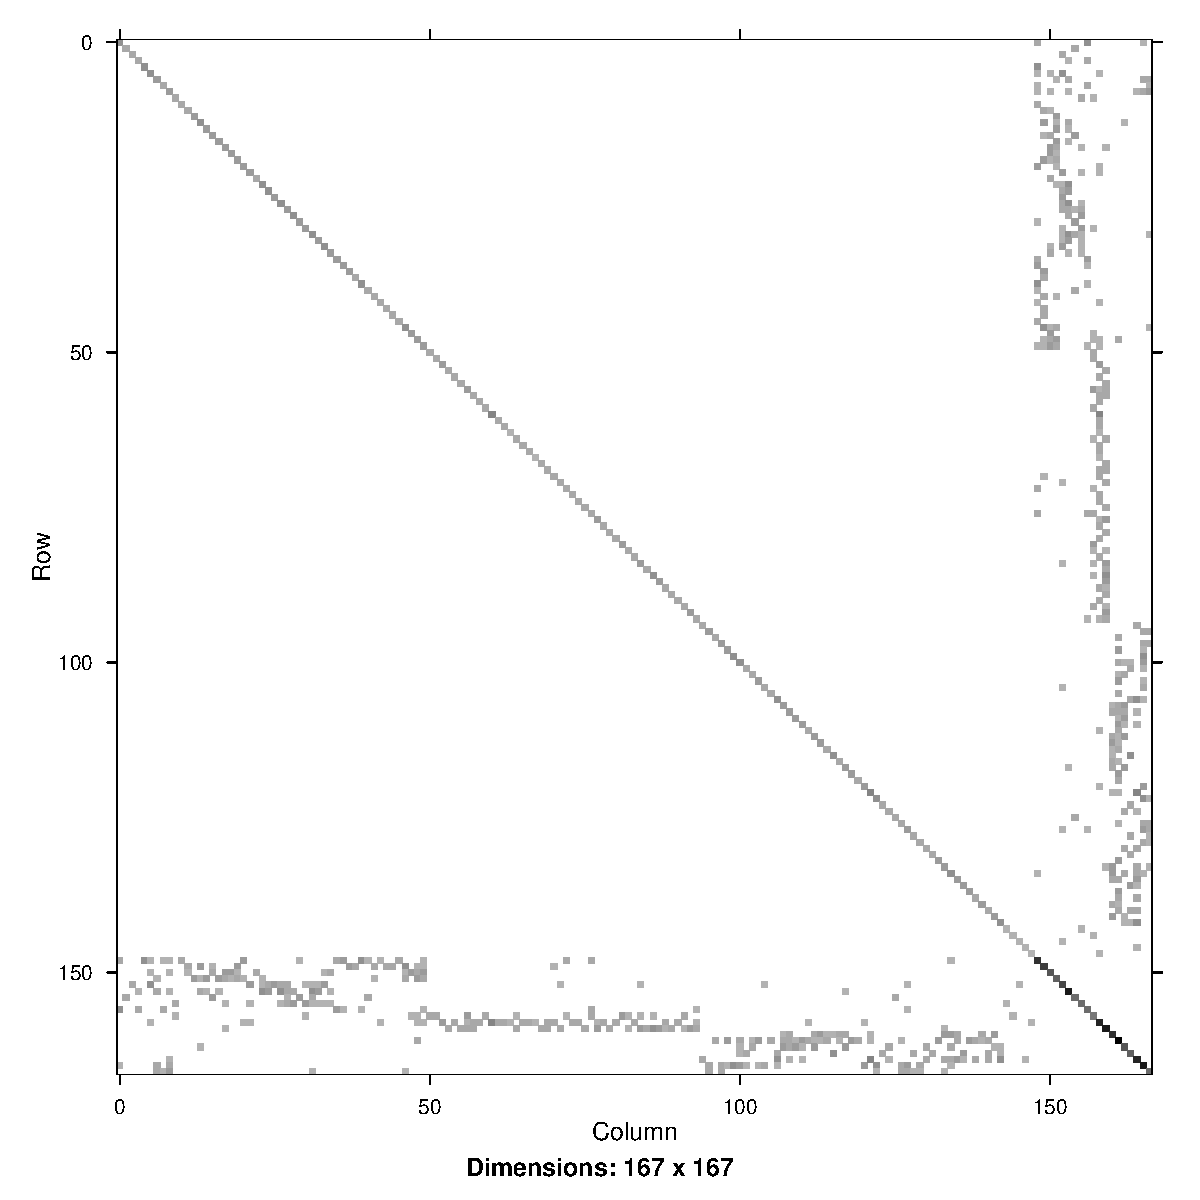
\includegraphics{MixedEffects-FigZtZ}
\caption{Location of nonzero elements in
  $\bZ\trans\bZ$ for a variance components model for the
  \var{ScotsSec} data.  Darker squares indicate larger magnitudes.
  Rows and columns are numbered from zero.  The first 148 rows and
  columns correspond to the levels of the \var{primary} grouping
  factor and the last 19 rows and columns correspond to levels of the
  \var{second} grouping factor.}
  \label{fig:ZtZ}
\end{figure}
for a variance components model using these grouping factors.

\subsubsection{General structure of the sparse matrix}
\label{ssec:Sparse}

For the variance components model $\bZ\trans\bZ$ is based on the
pairwise crosstabulation of the grouping factors.  In the more general
model, where some of the $\bZ_i$ can have multiple columns, the
structure of $\bZ\trans\bZ$ can be derived from the structure of the
pairwise crosstabulation matrix.  Both $\bZ\trans\bZ$ and the pairwise
crosstabulation can be divided into a $k\times k$ grid of blocks.  The
pattern of nonzeros in the $(i,j)$ block of $\bZ\trans\bZ$ is
obtained by replacing each nonzero in the $(i,j)$ block of the
crosstabulation by a $q_i\times q_j$ matrix.  Notice that we can
determine the patterns of nonzeros in $\bZ\trans\bZ$ knowing only the
$q_i,i=1,\dots,k$ and the pairwise crosstabulation of the grouping
factors.

\subsubsection{Crossed and nested grouping factors}
\label{ssec:Crossed}

In the Scottish secondary school example if all the students from a
given primary school attended the same secondary school we would say
that \var{primary} is \emph{nested within} \var{second}.  That is not
the case.  We can see in Figure~\ref{fig:ZtZ} that there is a moderate
amount of \emph{crossing} of these two grouping factors.  If there was
at least one student in the study from each combination of primary
school and secondary school we would describe the grouping factors
\var{primary} and \var{second} as being \emph{fully crossed}.  Again,
that is not the case for the Scottish secondary data.  Grouping
factors like these, which are neither nested nor fully crossed, are
said to be \emph{partially crossed}.

\subsection{Estimation criteria and related quantities}
\label{ssec:ModelCriteria}

For ease of reference we restate some of the results from
\citet{bate:debr:2004} in the form in which they will be calculated.

Given the observed responses $\by$ and the model matrices $\bX$ and
$\bZ$, we wish to determine either the maximum likelihood (ML) or the
restricted maximum likelihood (REML) estimates of the parameters
$\btheta$, $\bbeta$, and $\sigma^2$.  Because the conditional
estimates of $\bbeta$ and $\sigma^2$, given a value of $\btheta$, for
either criterion can be determined from the solution to a penalized
least squares problem, we can reduce the optimization problem to one
involving $\btheta$ only.  This reduction of the dimension of the
optimization problem is called \emph{profiling} the objective.

The conditional, penalized least squares problem can be solved using
the Cholesky decomposition
\begin{equation}
  \label{eq:CrossProdGen}
  \begin{bmatrix}
    \bZ\trans\bZ+\bOmega & \bZ\trans\bX  & \bZ\trans\by \\
    \bX\trans\bZ         & \bX\trans\bX  & \bX\trans\by \\
    \by\trans\bZ         & \by\trans\bX  & \by\trans\by
  \end{bmatrix}=\bR\trans\bR\quad\text{where}\quad\bR=
  \begin{bmatrix}
    \RZZ & \RZX & \rZy \\
    \bzer    & \RXX & \rXy \\
    \bzer    & \bzer    & \ryy
  \end{bmatrix} .
\end{equation}
The matrices $\RZZ$ and $\RXX$ are upper triangular of dimension
$q\times q$ and $p\times p$ respectively.  The corresponding vectors,
$\rZy$ and $\rXy$, are of dimension $q$ and $p$, and $\ryy$ is a
scalar.  The conditions that $\bOmega$ be positive definite and $\bX$
have full column rank ensure that $\RZZ$ and $\RXX$ are nonsingular.

In our implementation we do not form the upper triangular Cholesky
factor $\RZZ$.  Instead we use Tim Davis's LDL
package~\citep{Davis:2004} to factor
\begin{equation}
  \label{eq:LDLfactor}
  \bZ\trans\bZ+\bOmega=\bL\bD\bL\trans
\end{equation}
where $\bL$ is a sparse, unit, lower triangular matrix and $\bD$ is
diagonal with positive diagonal elements. Because the diagonal
elements of the unit triangular matrix $\bL$ are, by definition,
unity, they are not explicitly stored.

In general the matrices $\bZ\trans\bX$ and $\bX\trans\bX$ are dense.
We use functions from the LDL package to solve for $\RZX$ in
\begin{equation}
  \label{eq:RZX}
  \bD^{1/2}\bL\trans\RZX=\bZ\trans\bX
\end{equation}
Having solved for $\RZX$ we can downdate $\bX\trans\bX$ and determine
the dense upper triangular Cholesky factor $\RXX$ satisfying
\begin{equation}
  \label{eq:RXX}
  \RXX\trans\RXX=\bX\trans\bX-\RZX\trans\RZX
\end{equation}
Similar relationships are used to determine $\rZy$, $\rXy$, and
$\ryy$.  In fact, in our implementation we append $\by$ to $\bX$ when
forming $\bZ\trans\bX$ and $\bX\trans\bX$ so that
(\ref{eq:RZX}) provides both $\RZX$ and $\rZy$ and
(\ref{eq:RXX}) provides $\RXX$, $\rXy$, and $\ryy$.

The conditional estimates of $\bbeta$ satisfy
\begin{equation}
  \label{eq:betaHat}
  \RXX\widehat{\bbeta}(\btheta)=\rXy
\end{equation}
and the conditional modes of the random effects satisfy
\begin{equation}
  \label{eq:ConditionalExp}
  \bD^{1/2}\bL\trans\widehat{\bb}(\btheta)=\rZy-\RZX\widehat{\bbeta} .
\end{equation}
The conditional ML estimate of $\sigma^2$ is
$\widehat{\sigma^2}(\btheta)=\ryy^2/n$ and the conditional REML
estimate is $\widehat{\sigma^2}_R(\btheta)=\ryy^2/(n-p)$.

The profiled optimization problem, expressed in terms of the
deviance, is
\begin{equation}
  \label{eq:ProfiledLogLik}
  \begin{aligned}
    \widehat{\btheta}&=\arg\min_{\btheta} -2\tilde{\ell}(\btheta)\\
    &=\arg\min_{\btheta}\left\{\log\left(\frac{\left|\bD\right|}
      {\left|\bOmega\right|}\right)
    + n\left[1+\log\left(\frac{2\pi\ryy^2}{n}\right)\right]\right\}
  \end{aligned}
\end{equation}
\begin{equation}
  \label{eq:ProfiledLogRestLik}
  \begin{aligned}
    \widehat{\btheta_R}&=\arg\min_{\btheta} -2\tilde{\ell_R}(\btheta)\\
    &=\arg\min_{\btheta}\left\{\log\left(\frac{\left|\bD\right|\left|\RXX\right|^2}
      {\left|\bOmega\right|}\right)
    +  (n-p)\left[1+\log\left(\frac{2\pi\ryy^2}{n-p}\right)\right]\right\}
  \end{aligned}
\end{equation}
for ML and REML estimation, respectively.  The gradients of these
criteria are
\begin{align}
  \label{eq:gradDev}
  \nabla(-2\tilde\ell)&=\tr\left[\der\bOmega\left(
      (\bZ\trans\bZ+\bOmega)^{-1}-\bOmega^{-1}+
      \frac{\widehat{\bb}}{\widehat{\sigma}}
      \frac{\widehat{\bb}}{\widehat{\sigma}}\trans\right)\right]\\
  \label{eq:gradDevRest}
  \nabla(-2\tilde\ell_R)&=\tr\left[\der\bOmega\left(
      \vb-\bOmega^{-1}+
      \frac{\widehat{\bb}}{\widehat{\sigma}_R}
      \frac{\widehat{\bb}}{\widehat{\sigma}_R}\trans\right)\right]
\end{align}
where
\begin{equation}
  \label{eq:vbDef}
  \vb=\bL\invtrans\bD^{-1/2}\left(\bI+\RZX\RXX^{-1}\RXX\invtrans
    \RZX\trans\right)\bD^{-1/2}\bL^{-1}
\end{equation}
and $\der$ denotes the Frechet derivative.

If good starting estimates of $\btheta$ are not available, the initial
Newton iterations for (\ref{eq:ProfiledLogLik}) or
(\ref{eq:ProfiledLogRestLik}) can be unstable.  We can refine our
initial estimates with a moderate number of ECME steps
for which $\btheta_{i+1}$ satisfies
\begin{equation}
  \label{eq:theta1}
  \tr\left[\der\bOmega\left(
      \frac{\widehat{\bb}(\btheta_i)}{\widehat{\sigma}(\btheta_{i})}
      \frac{\widehat{\bb}(\btheta_i)\trans}{\widehat{\sigma}(\btheta_{i})}+
      \left(\bZ\trans\bZ+\bOmega(\btheta_{i})\right)^{-1}
      -\bOmega(\btheta_{i+1})^{-1}\right)\right]=\bzer
\end{equation}
for ML estimates or
\begin{equation}
  \label{eq:theta1R}
  \tr\left[\der\bOmega\left(
      \frac{\widehat{\bb}(\btheta_{i})}{\widehat{\sigma}_R(\btheta_i)}
      \frac{\widehat{\bb}(\btheta_{i})\trans}{\widehat{\sigma}_R(\btheta_i)}+
      \vb(\btheta_{i})
      -\bOmega(\btheta_{i+1})^{-1}\right)\right]=\bzer
\end{equation}
for REML.

At this point it is easy to formulate a general method of obtaining ML
or REML estimates for a linear mixed model:
\begin{enumerate}
\item Given the data $\by$ and the model matrices $\bX$ and $\bZ$,
  formulate initial estimates $\btheta_0$.  Some heuristics for doing
  so are given in \citet[ch.~3]{pinh:bate:2000}.
\item Use a moderate number of ECME steps, (\ref{eq:theta1}) or
  (\ref{eq:theta1R}), to refine these starting estimates.  Each ECME
  step requires evaluating $\bOmega(\btheta)$ followed by the
  decomposition (\ref{eq:CrossProdGen}) and the solutions to (\ref{eq:RZX}),
  (\ref{eq:RXX}), (\ref{eq:betaHat}) and (\ref{eq:ConditionalExp}).
\item Use a Newton method to optimize the criterion
  (\ref{eq:ProfiledLogLik}) or (\ref{eq:ProfiledLogRestLik}) with
  gradient (\ref{eq:gradDev}) or (\ref{eq:gradDevRest}).  Each
  evaluation of the criterion requires evaluating $\bOmega(\btheta)$
  followed by the decomposition (\ref{eq:CrossProdGen}) and the
  solutions to (\ref{eq:RZX}) and (\ref{eq:RXX}).  Gradient
  evaluations require the solutions to (\ref{eq:betaHat}) and
  (\ref{eq:ConditionalExp}).
\end{enumerate}
In \citet{bate:debr:2004} we show that similar calculations can be
used to evaluate the Hessian of the profiled criteria and that the
deviance forms of the criteria are bounded below throughout the
parameter space.  Reasonable starting values determined by
the ECME iterations and analytic expressions for the gradients and
Hessians help to make (\ref{eq:ProfiledLogLik}) and
(\ref{eq:ProfiledLogRestLik}) very well controlled optimization
problems.  The most difficult computational step in the ECME or Newton
iterations is the sparse Cholesky decomposition (\ref{eq:CrossProdGen}).

\section{Symbolic analysis}
\label{sec:Symbolic}

Although the decomposition (\ref{eq:CrossProdGen}) will be performed
many times for different trial values of $\btheta$, the structure of
$\bZ\trans\bZ+\bOmega$ -- in particular, the number and the positions of
nonzeros in $\bZ\trans\bZ+\bOmega$ and in $\bL$ -- will be the
same for each evaluation.  Because the LDL package provides one
function to perform the symbolic analysis and another function to
determine the numerical values in the decomposition, we can do
the symbolic analysis separately.

The number and the positions of the nonzeros in $\bL$ depend on the
positions of the nonzeros in $\bZ\trans\bZ$. Any nonzero position in
the lower triangle of $\bZ\trans\bZ$ can be nonzero in $\bL$.
However other positions in $\bL$ can become nonzero during the course
of the decomposition.  This is called ``fill-in''.  The extent of the
fill-in can be altered by reordering the components of $\bb$ (and
correspondingly the columns of $\bZ$).

Although there are general approaches, such as approximate minimal
degree~\citep{Davis:1996} or graph-partitioning
algorithms~\citep{Metis}, for determining a fill-minimizing
permutation, it is more effective for us to exploit the special
structure of $\bZ\trans\bZ$ in searching for such a permutation.

As mentioned above, when considering the structure of
$\bZ\trans\bZ+\bOmega$ we need only consider the structure for the
variance components model because the structure for the general model
is obtained from the structure for the variance components model by
replacing each nonzero in the $(i,j)$ block of the variance components
model by a $q_i\times q_j$ nonzero matrix.  Similarly we can derive
the structure of the $\bL$ matrix for the general model from that of
the variance components model provided we restrict our attention to
permutations that do not mix levels from different grouping factors.
That is, we consider only those fill-reducing permutations that
consist of, at most, a permutation of the grouping factors and
permutations of the levels within each grouping factor.  Note that we
can determine such a permutation based only on the pairwise
crosstabulation of the grouping factors.  That is, the
fill-reducing permutation for the variance components model provides
the fill-reducing permutation for the general model.  Hence, in what
follows, we consider only the variance components model.

Fill-in is determined by the elimination tree~\citep{Liu:1990} for the
symmetric matrix.  We can determine the Cholesky decomposition, and
hence the elimination tree and the extent of the fill-in, column-wise
starting with the first column.  We know that there will be
``original'' nonzeros in $\bL$ wherever there are nonzeros in the
lower triangle of $\bZ\trans\bZ+\bOmega$ and, possibly, some
additional, ``induced'' nonzeros.  If there are nonzeros, either
original or induced, below the diagonal in column $j$, say in rows
$i$ and $k$, then a nonzero is induced in the $(i,k)$ position of
$\bL$.  Consider again the division of $\bZ\trans\bZ+\bOmega$ and
$\bL$ into a $k\times k$ array of blocks determined by the grouping
factors.  For a variance components model, the diagonal blocks are
themselves diagonal.  Because the $(1,1)$ block is diagonal the row
numbers of any nonzeros below the diagonal must be greater than $m_1$.
That is, there will not be any induced nonzeros in the first $m_1$
columns. Because this first block of $m_1$ rows and columns will not
experience any fill-in, we choose the first grouping factor to have
the greatest number of levels.  In general we order the grouping
factors so that $m_1\ge m_2\ge\dots\ge m_k$.

There is no need to permute the levels of the first grouping
factor, which can result in a considerable savings in the effort required to
determine a fill-reducing permutation.  For the Scottish secondary
school example we can leave the first 148 columns in their original
order and consider only permutations of the last 19 columns.

We obtain the matrix to determine the permutation of the second and
subsequent groups by ``projecting'' the first $m_1$ columns onto the
last $q-m_1$ columns.  If there are only two
grouping factors we record as potentially nonzero the positions $(i,k)$
with $i,k>m_1$ and both $(i,j)$ and $(k,j)$ nonzero for some
$j\le m_1$.  If there are more than two grouping factors we
record all these positions plus any of the original nonzeros below the
$m_1$st row and to the right of the $m_1$st column.

In the case of two nested grouping factors there will only be one
nonzero element below the diagonal in each of the first $m_1$ columns,
hence there is no fill-in.  For more than two nested grouping factors,
any pair of nonzeros occuring in the first $m_1$ columns must be in
rows associated with different grouping factors and, furthermore, the
nonzero off-diagonal that would be generated in the projected matrix
for that combination must already be nonzero.  That is, nested
grouping factors do not generate any fill-in.  Not only can the matrix
$\bL$ be created ``in place'' (that is, with exactly the same
positions of nonzeros as in the lower triangle of $\bZ\trans\bZ$) but
also $\bL^{-1}$ has the same pattern of nonzeros.  This is unusual.
In most cases $\bL^{-1}$ has many more nonzeros than does $\bL$.

Notice that a single grouping factor is, trivially, a nested sequence.


\subsection{Examples}
\label{ssec:ProjectionEx}

In Figure~\ref{fig:ScotsProj} we show the projection of the symmetric
matrix in Figure~\ref{fig:ZtZ} onto the $19\times19$ block for the
\var{second} factor.
\begin{figure}[tbp]
  \centering
\setkeys{Gin}{width=\textwidth}
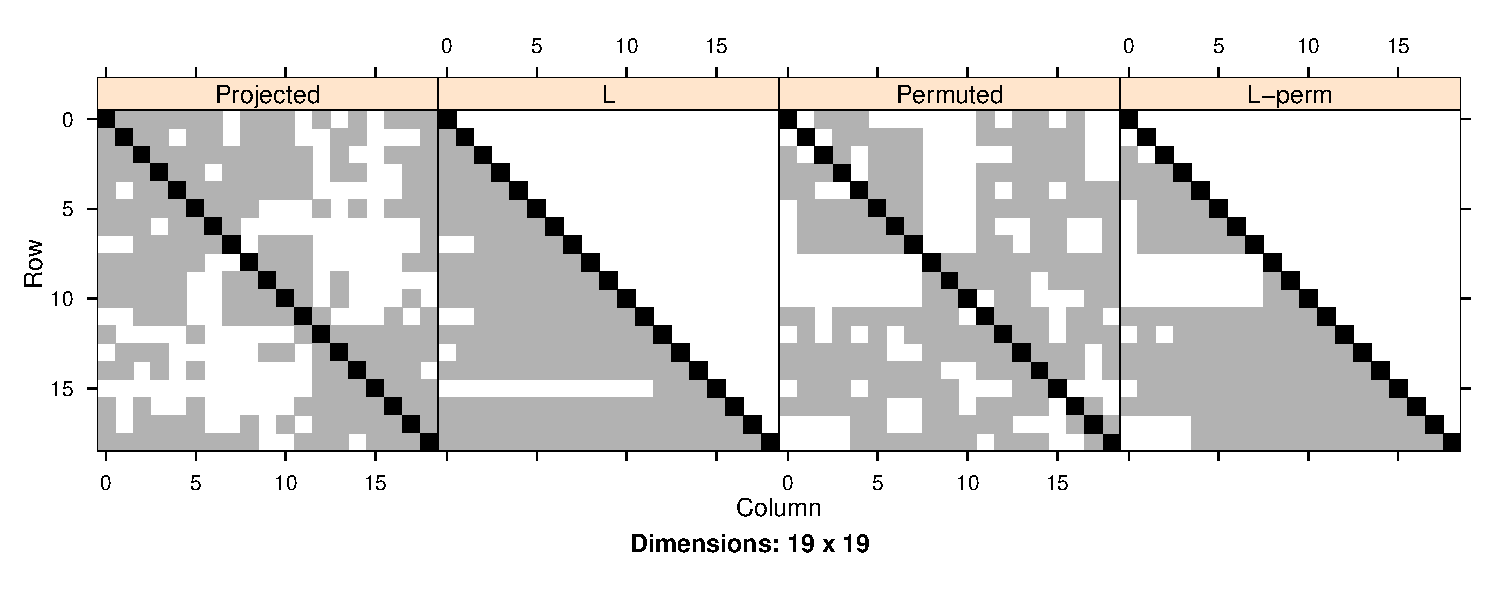
\includegraphics{MixedEffects-FigScotsProj}
  \caption{Projection of the pairwise crosstabulation for the Scottish
    secondary school data onto the $19\times 19$ lower right block for
    the \var{second} factor.  The ``Projected'' panel shows the
    original (black squares) and projected (gray squares) nonzero
    positions.  The ``L'' panel shows the implicit diagonal (black
    squares) and the nonzero off-diagonal (gray squares) for this
    ordering of the levels of the factor.  The ``Permuted'' panel
    shows the symmetric matrix after permuting the rows and columns
    according to the fill-reducing permutation determined by the Metis
    package and the ``L-perm'' panel shows the $\bL$ matrix from this
    ordering.}
  \label{fig:ScotsProj}
\end{figure}
We also show the patterns of nonzeros in $\bL$ from the LDL
decomposition of this block (using the original ordering of the rows and
columns); the symmetric block with its rows and columns permuted
according to a fill-reducing permutation determined by
Metis~\citep{Metis}; and the nonzeros in the $\bL$ matrix from the
decomposition of the permuted symmetric matrix.

In this case the fill-minimizing permutation does not produce a great
savings in the amount of storage, even relative to dense storage of
the matrix which would have 171 elements below the diagonal.
Without the fill-minimizing permutation there are 154 off-diagonal
nonzeros in $\bL$.  With the permutation there are 131.

Even so, only 470 floating point values are required to store
$\bZ\trans\bZ$ and a total of 601 for the decomposition (167 for $\bD$
and 434 for $\bL$).  Dense storage of the $(2,1)$ block of
$\bZ\trans\bZ$, as suggested in \citet{MLwiN:2002}, would require 2812
floating point locations for that block alone, plus a similar number
for the decomposition.  In this example it is the sparse storage, more
than the fill-reducing permutation, that reduces both the space and the
computational time required, relative to previous methods.

In other cases, however, the storage savings from the fill-reducing
permutation can be substantial.  We have used these methods to analyze
378,047 test scores of 134,713 students in 3722 schools.  There are
377,111 nonredundant nonzeros in the pairwise crosstabulation (138,435
diagonals and 238,676 off-diagonals).  The projection of the $(2,1)$
block into the $(2,2)$ block produces a symmetric $3722\times 3722$
matrix with 49,305 non-redundant nonzeros (3722 diagonals and 45,583
off-diagonals).  Without the fill-reducing permutation the $\bL$
matrix has 4,469,124 nonzero off-diagonals or 64.5\% of the maximum
possible number (6,924,781). With the permutation the number of
nonzero off-diagonals is reduced to 193,562 or 2.8\% of the maximum.

Fitting linear mixed models to data, such as these, that have a large
number of levels in one or more of a set of partially crossed grouping
factors has been very difficult, if not impossible, with existing
multilevel modeling software.  Using a dense representation of the
$(2,1)$ block (over $5\times 10^8$ floating point values or 4 GB per
copy, in double precision) is impractical on most current computers.  A
sparse matrix representation combined with a fill-reducing permutation
makes it practical to perform multilevel analysis of such data, which is
becoming common~\citep{Rnews:Lockwood+Doran+Mccaffrey:2003}.

\section{Generalizations of linear mixed models}
\label{sec:Generalizations}

A generalized linear mixed model is similar to a linear mixed model
except that the linear predictor
\begin{equation}
  \label{eq:GLMMlinpred}
  \boeta = \bX\bbeta+\bZ\bb = g(\bmu)
\end{equation}
is a function $g$, called the \emph{link} function, of the mean
vector, $\bmu$.  Furthermore, the conditional density of the
responses, $p(\by|\bbeta,\bb,\btheta)$, may be other than Gaussian.

Usually the conditional density is a member of the exponential family,
such as the Bernoulli distribution for binary responses or the Poisson
distribution for count data, in which case there is a canonical link function
(the logit link for the Bernoulli and the log link for the Poisson).

In many cases, such as the Bernoulli and the Poisson, the conditional
distribution of the response depends only on the mean.  In other
cases, such as the Gaussian and gamma distributions, there is a
(common) scale parameter in the distribution.  If there is a scale
parameter we incorporate it in the general dispersion parameter $\btheta$.

\citet{mccullagh:nelder:1989} describe an iteratively reweighted least
squares (IRLS) algorithm for determining the MLEs of the coefficients
$\bbeta$ and, if used, the scale parameter, in a generalized linear
model without random effects.  A penalized quasi-likelihood (PQL)
algorithm for estimation of the parameters in a GLMM can be
implemented by replacing the least squares problem in IRLS by the penalized
least squares (PLS) problem represented by (\ref{eq:CrossProdGen}).
Within each of the IRLS iterations, we perform some ECME and/or Newton
iterations to optimize the log-likelihood (as a function of $\btheta$)
represented by the PLS problem.  Convergence of this PQL algorithm is
indicated by its reaching a stationary point.

Thus the techniques described in \S\ref{sec:LinearMixed} and
\S\ref{sec:Symbolic} provide the inner optimization for the PQL
algorithm.  Although PQL is not guaranteed to produce the maximum
likelihood estimators of the parameters $\bbeta$ and $\btheta$, it
will generally get close to the MLEs.  After PQL has converged we
switch to direct optimization of the marginal likelihood
\begin{equation}
  \label{eq:likelihood}
  L(\bbeta,\btheta)=\int_{\bb} p(\by|\bbeta,\bb,\btheta)
  p(\bb|\btheta)\,d\bb .
\end{equation}

The integral (\ref{eq:likelihood}) does not, in general, have a closed
form.  Two effective ways of approximating this integral are Laplacian
integration~\citep{tier:kada:1986} and adaptive Gauss-Hermite
integration~\citep{pinh:bate:2000} for which the conditional modes of
the random effects
\begin{equation}
  \label{eq:CondModes}
  \widehat{\bb}(\bbeta,\btheta)=
  \arg\max_{\bb} p(\by|\bbeta,\bb,\btheta)p(\bb,\btheta)
\end{equation}
are required.

The conditional modes can be determined by a penalized IRLS algorithm
implemented using the representations and decompositions described in
\S\ref{sec:LinearMixed} and \S\ref{sec:Symbolic}.


\subsection{Nonlinear mixed models}
\label{ssec:NMM}

In a nonlinear mixed model element $i$ of the expected response
$\mathrm{E}[\bY]$ is a function of covariates $\bx_i$ associated with
that observed response and a $r$-dimensional parameter $\bphi_i$.
\begin{equation}
  \label{eq:NMM}
  \left\{\mathrm{E}[\bY]\right\}_i = f(\bphi_i, \bx_i)\quad
  i=1,\dots,n .
\end{equation}
The values of $\bphi$ can be represented as an $n\times r$ matrix $\bPhi$.
Each column of this matrix is a linear function of $\bbeta$ and $\bb$
\begin{equation}
  \label{eq:NMMcomp}
  \bPhi_j=\bX_j\bbeta+\bZ_j\bb\quad j=1,\dots,r
\end{equation}

If the function $f$ is linear in all the elements of $\bphi_i$ the NMM
can be reexpressed as a LMM, hence we will assume that $f$ is
nonlinear in at least one of these elements.

For a fixed value of $\btheta$ we can express the conditional
estimates of the fixed effects $\bbeta$ and the condtional modes of
the random effects as the solution to a penalized nonlinear least
squares (PNLS) problem.  The algorithm proposed in
\citet{lind:bate:1990} is essentially the the same as the PQL algorithm for generalized linear models but with the PIRLS
step replaced by PNLS.  Just like PQL this algorithm will generally
get close to the MLEs but does not produce the exact MLEs except in
special circumstances.  

Estimates obtained by maximizing the Laplacian approximation or an
adaptive Gauss-Hermite approximation to the marginal likelihood should
be closer to the MLEs.  As in the case of the GLMM these
approximations require the conditional modes of the random effects.
These are the solutions to a penalized nonlinear least squares problem
for which the representation and decompositions described in
\S\ref{sec:LinearMixed} and \S\ref{sec:Symbolic} can be used.

\section{Implementation}
\label{sec:Implementation}

The techniques described in \S\ref{sec:LinearMixed} and
\S\ref{sec:Symbolic} for linear mixed models, and the PQL and Laplace
methods for generalized linear mixed models are currently implemented
in the \code{lme4} package for R~\citep{R-2.0.0}.  In future versions
of this package we will incorporate the adaptive Gauss-Hermite method
for GLMMs and the PQL, Laplace, and adaptive Gauss-Hermite methods for
NMMs.

Because both R and the \code{lme4} package are open source software,
they provide a reference implementation of these methods against which
other methods can be compared.  However, the package is more than a
``reference implementation''; it is carefully implemented and is
suitable as a production system.  As part of the package we provide a
``vignette'' (a code/documentation combination for literate data
analysis) that fits the models from the examples in the comparative
reviews of multilevel modeling software
(\url{http://multilevel.ioe.ac.uk/softrev/}).  These examples show
that the \code{lme} function in the \code{lme4} package is fast and
reliable on what would currently be considered typical multilevel
modeling examples.  However, the sparse matrix representation and the
ease of model specification allows it to go far beyond currently
available software.  We know of no other software that can fit models
with partially crossed grouping factors to data sets with $10^5$ or
more observations, such as the longitudinal analysis of over 300,000
test scores described in \S\ref{ssec:ProjectionEx} incorporating
random effects for student and school and allowing for student
migration between schools.

\section{Conclusions}
\label{sec:Summary}

We have presented a specification of linear mixed models using model
matrices and grouping factors, a computational representation based
this specification, computational methods using the representation,
and, to a lesser extent, described an implementation of the
specification, representation, and computational methods.
Furthermore, we show that the specification, representation, methods,
and implementation can be extended to generalizations of the linear
mixed model including GLMMs and NMMs.

Specification of the model is important.  In many software
implementations of methods for fitting linear mixed models it can be
awkward to specify the structure of the random effects.  We contend
that by concentrating on the grouping factors in the data and on the
model matrices associated with these grouping factors, the
specification of linear mixed models is made much easier.  Nesting or
crossing of grouping factors can be determined from the data, rather
than having to be specified as part of the model.  Common forms of
linear mixed models (including all those in the comparative review of
multilevel modeling software,
\url{http://multilevel.ioe.ac.uk/softrev/}) can be specified without
using specialized forms of the precision matrices $\bOmega_i,
i=1,\dots,k$.  We only require that these matrices are symmetric and
positive definite, which makes the implementation much simpler because
we do not need to work with esoteric forms of precision matrices, or
variance-covariance matrices, for the random effects.

A pairwise crosstabulation of the grouping factors, which we store as
a sparse symmetric matrix, is the basis of all the symbolic analysis.
Even when some of the $q_i>1$ we can do all the symbolic analysis on
the crosstabulation without needing the model matrices.  It is only
when the numeric representation is being formed that we need the model
matrices.  Because the number of nonzero elements in the LDL
decomposition is determined during the symbolic analysis we can
allocate all the storage needed for later calculations immediately
after this stage.

We can ``project out'' the effect of the first grouping factor on the
reordering of the columns of the matrix $\bZ$.  Because it is common
for the number of levels in one of the grouping factors to be
comparable to the number of observations, ordering the grouping
factors so that $m1\ge m2\ge\dots\ge m_k$ can simplify the symbolic
analysis considerably.

The representation provided by the sparse symmetric storage of
$\bZ\trans\bZ$ and the dense storage of $\bZ\trans\bX$ and
$\bX\trans\bX$ (where $\bX$ actually contains both $\bX$ and $\by$),
provides a remarkably efficient means of evaluating the profiled
log-likelihood and restricted log-likelihood.  ECME
iterative steps can be efficiently implemented with this
representation.  After a moderate number of ECME steps it is advantageous
to switch to a Newton or quasi-Newton optimization method, for
which the gradient and, optionally, the Hessian of the objective can
be evaluated.

\section{Acknowledgements}
\label{sec:Ack}

This work was supported by U.S.{} Army Medical Research and Materiel
Command under Contract No.{} DAMD17-02-C-0119.  The views, opinions
and/or findings contained in this report are those of the authors and
should not be construed as an official Department of the Army
position, policy or decision unless so designated by other
documentation.

I thank Deepayan Sarkar and Tim Davis for helpful discussions and
suggestions and Harold Doran for his suggestion of using sparse
matrix techniques for linear mixed-effects models.

The \code{Matrix} package for \RR{} is based on code from the
LDL~\citep{Davis:2004}, TAUCS~\citep{Taucs}, and Metis~\citep{Metis}
packages.

\bibliography{lme4}
\end{document}

\section{Sparse matrix classes and methods in the Matrix package for R}
\label{sec:SparseM}

The simplest representation of a sparse matrix $\bX$ is to store a
triplet $(i,j,x_{ij})$ for each nonzero element.  If the triplets are
sorted, say by column order, the column indices will occur in blocks
of equal values.  In the \emph{compressed, sparse, column-oriented}
format the entries are sorted in increasing column order and a set of
pointers to the beginning of each column are used instead of the
column values themselves.  The \var{tripletMatrix} class in the
\var{Matrix} package provides the triplet format and the
\var{cscMatrix} class provides the compressed, sparse column-oriented
format.  In both these classes indices are 0-based (for compatibility
with the underlying C code) and not 1-based as is common in R.
\begin{Schunk}
\begin{Sinput}
> library(Matrix)
> mm = new("tripletMatrix", i = as(c(0, 2, 3, 1, 2, 0, 3, 4, 
+     3, 4), "integer"), j = as(c(0, 0, 0, 1, 1, 2, 2, 2, 3, 
+     3), "integer"), x = (1:10)/10, Dim = as(c(5, 4), "integer"))
> m1 = as(mm, "cscMatrix")
> str(m1)
\end{Sinput}
\begin{Soutput}
Formal class 'cscMatrix' [package "Matrix"] with 5 slots
  ..@ p            : int [1:5] 0 3 5 8 10
  ..@ i            : int [1:10] 0 2 3 1 2 0 3 4 3 4
  ..@ x            : num [1:10] 0.1 0.2 0.3 0.4 0.5 0.6 0.7 0.8 0.9 1
  ..@ Dim          : int [1:2] 5 4
  ..@ factorization: list()
\end{Soutput}
\begin{Sinput}
> as(m1, "matrix")
\end{Sinput}
\begin{Soutput}
     [,1] [,2] [,3] [,4]
[1,]  0.1  0.0  0.6  0.0
[2,]  0.0  0.4  0.0  0.0
[3,]  0.2  0.5  0.0  0.0
[4,]  0.3  0.0  0.7  0.9
[5,]  0.0  0.0  0.8  1.0
\end{Soutput}
\begin{Sinput}
> diff(m1@p)
\end{Sinput}
\begin{Soutput}
[1] 3 2 3 2
\end{Soutput}
\end{Schunk}
We see that the \var{p} slot in a \var{cscMatrix} with 4 columns has 5
elements.  The first element is always zero and the successive differences
are the numbers of nonzero elements in each column.  The total number
of nonzero elements is the value of the last element of the \var{p}
slot.  This is also the length of the vector of row indices in the
\var{i} slot.

The validation method for the \var{cscMatrix} class ensures that the
row indices are increasing within columns and reorders the \var{i} and
\var{x} slots if necessary to achieve this.  Technically, the objects
in this class can be described as sorted, compressed, sparse,
column-oriented matrices.

Objects in the \var{tscMatrix} class represent triangular, sparse,
column-oriented matrices and those in the \var{sscMatrix} class
represent symmetric, sparse, column-oriented matrices.  Only the
upper triangle or the lower triangle, as indicated by \code{"U"} or
\code{"L"} in the \var{uplo} slot, of a symmetric matrix is stored.
The \var{crossprod} function applied to a \var{cscMatrix} produces an
\var{sscMatrix}.
\begin{Schunk}
\begin{Sinput}
> class(m2 <- crossprod(m1))
\end{Sinput}
\begin{Soutput}
[1] "sscMatrix"
attr(,"package")
[1] "Matrix"
\end{Soutput}
\begin{Sinput}
> as(m2, "matrix")
\end{Sinput}
\begin{Soutput}
     [,1] [,2] [,3] [,4]
[1,] 0.14 0.00 0.00 0.00
[2,] 0.10 0.41 0.00 0.00
[3,] 0.27 0.00 1.49 0.00
[4,] 0.27 0.00 1.43 1.81
\end{Soutput}
\end{Schunk}

In Statistics we usually define the Cholesky decomposition of a
positive semidefinite, symmetric matrix $\bA$ as an upper triangular
matrix $\bR$ such that $\bA=\bR\trans\bR$ but it is also frequently
defined as a lower triangular matrix $\bL$ such that
$\bA=\bL\bL\trans$.  Naturally, $\bL$ and $\bR$ are transposes of each
other.  On occasion there are advantages to working with the left
factor $\bL$ instead of the right factor $\bR$.

For a sparse, symmetric, semidefinite matrix reordering the columns
(and, correspondingly, the rows) of $\bA$ can change the number of
nonzero elements in the Cholesky factor.  The number of elements in
the Cholesky factor is at least the number of nonzero elements in the
lower triangle of $\bA$.  Additional nonzeros can be generated during
the decomposition.  This process is called ``fill-in''.  Various
methods of determining a fill-minimizing order have been proposed.  We
use a graph-based method implemented in the Metis package.

The \var{chol} function generates the Cholesky decomposition.   When
applied to an \var{sscMatrix} object it defaults to generating a
fill-reducing permutation and the Cholesky factor of the permuted matrix.
\begin{Schunk}
\begin{Sinput}
> m3 = chol(m2)
> as(m3, "matrix")
\end{Sinput}
\begin{Soutput}
          [,1]       [,2]      [,3]      [,4]
[1,] 1.3453624 0.00000000 0.0000000 0.0000000
[2,] 1.0629106 0.60018413 0.0000000 0.0000000
[3,] 0.0000000 0.00000000 0.6403124 0.0000000
[4,] 0.2006894 0.09444615 0.1561738 0.2577080
\end{Soutput}
\begin{Sinput}
> m3@perm
\end{Sinput}
\begin{Soutput}
[1] 3 2 1 0
\end{Soutput}
\end{Schunk}
If we set the optional argument \var{pivot} to \var{FALSE},
calculation of the fill-reducing permutation is suppressed.
\begin{Schunk}
\begin{Sinput}
> as(chol(m2, pivot = FALSE), "matrix")
\end{Sinput}
\begin{Soutput}
          [,1]       [,2]      [,3]    [,4]
[1,] 0.3741657  0.0000000 0.0000000 0.00000
[2,] 0.2672612  0.5818689 0.0000000 0.00000
[3,] 0.7216054 -0.3314443 0.9270547 0.00000
[4,] 0.7216054 -0.3314443 0.8623336 0.66016
\end{Soutput}
\end{Schunk}
In this example the fill-reducing permutation reverses the order of
the columns and rows of \var{m2} before taking the decomposition.  It
results in two fewer nonzero elements in the decomposition than when
we suppress the permutation.

\subsection{Symbolic versus numeric computation}
\label{sec:symbolic}

Calculation of the fill-reducing ordering is an example of a symbolic
computation on sparse matrices in that it is based only on the
positions of the nonzero elements, not upon their values.  Frequently
a sparse-matrix computation has both a symbolic phase, which typically
determines the number and positions of the nonzero entries in the
result, and a numeric phase that actually calculates these nonzero
elements.

Evaluation of the profiled log-likelihood or profiled
log-restricted-likelihood requires updating the diagonal blocks in
$\bZ\trans\bZ$ and taking the Cholesky decomposition of the resulting
matrix.  The symbolic phases, including calculation of a fill-reducing
ordering only need to be done once.

Recently Tim Davis has released the LDL package that provides a
concise Cholesky factorization of the form $\bA=\bL\bD\bL\trans$ where
$\bL$ is a unit lower triangular matrix (i.e. all the diagonal
elements are unity) and $\bD$ is diagonal and stored as a single
vector.  This representation is particularly convenient for us because
the diagonal elements (which must be nonzero when $\bA$ is positive
definite) often constitute a substantial portion of the total number
of nonzero elements in the Cholesky factor and, in this
representations, we do not encounter the extra indexing overhead when
accessing these elements.  Also the determinant of $\bA$ (or, for our
purposes, the determinants of leading diagonal submatrices of $\bA$)
can be calculated directly from the diagonal of $\bD$.

In common models for such data
\citep{Rnews:Lockwood+Doran+Mccaffrey:2003}, the random effects are
associated with the primary school and the secondary school that the
student attended, which is to say that \var{primary}, with 148
distinct levels, and \var{second}, with 19 distinct levels, are the
grouping factors.  


We see that $\Omega$ has a very simple structure.  The matrix
$\bZ\trans\bZ$ is sparse but not as simple.  To determine its
structure we must first examine $\bZ$ which has 3435 rows
(corresponding to students) and 167 columns.  The first 148 columns
are the indicators of the primary schools.  That is, if student $i$
attended primary school $j$ then
\begin{equation}
  \label{eq:bZik}
  \{\bZ\}_{ik}=
  \begin{cases}
    1&k=j\\
    0&k\ne j
  \end{cases}
\end{equation}
The last 19 columns are the indicators of the secondary schools.
The diagonal elements of $\bZ\trans\bZ$ are the tabulation of the
number of students attending each primary school followed by the
number of students attending each secondary school.  Part of this
tabulation is given in the output of the \var{summary} function above.
Here we give the full tabulation of the secondary schools and part of
the crosstabulation of the primary and secondary schools.
\begin{Schunk}
\begin{Sinput}
> xtabs(~second, ScotsSec)
\end{Sinput}
\begin{Soutput}
second
  1   2   3   4   5   6   7   8   9  10  11  12  13  14  15  16  17  18 
219 199 156 139 175 250 109 107 114  92 234 253 216 290 147 134 233 257 
 19 
111 
\end{Soutput}
\end{Schunk}

For the purposes of this study each student is classified as attending
only one primary school and one secondary school.  Primary school $i$
can occur with secondary school $j$ but not all of these combinations
do 
one prim
but one of these columns, the column corresponding to the primary school
There is a corresponding grouping of the columns of the matrix $\bZ$
into $m_1\times q_1$ columns associated with the first grouping factor
$\bff_1$, $m_2\times q_2$ columns associated with the second grouping
factor $\bff_2$, and so on.  A given observation, corresponding to a
row of $\bZ$, is associated with exactly one level of $\bff_1$, one
level of $\bff_2$, and so on and all the elements of that row of $\bZ$
will be zero except for the corresponding $q_1$ columns in the first
group, the corresponding $q_2$ columns in the second group, and so on.

This structure in $\bZ$ induces a special structure in $\bZ\trans\bZ$.
It is symmetric and can be divided into $k\times k$ ``outer blocks'',
corresponding to the $k$ grouping factors. The $(i,j)$ outer block, of
size $m_i q_i\times m_j q_j$, is further subdivided into $m_i\times
m_j$ inner blocks, each of size $q_i\times q_j$.  The $(m,n)$'th inner
block in the $(i,j)$'th outer block will be nonzero only if level $m$
of $\bff_i$ occurs with level $n$ of $\bff_j$.  In particular, a
diagonal outer block is block-diagonal with the diagonal consisting of
$m_i$ (possibly different) blocks of size $q_i\times q_i$.

As discussed later, $\bOmega$ has a block diagonal structure and its
determinant is easily evaluated.  The determinant
$\left|\bZ\trans\bZ+\bOmega\right|$ is the product of the elements of
$\dZ$ and $\left|\LXX\right|^2$ is the product of the elements of $\dX$.

The other results given in \citet{bate:debr:2004} can be calculated
from $\bL$ and $\bD$.  To make all this feasible the structure and, in
particular, the sparsity of $\bZ$ and $\bOmega$ must be exploited.

Sparsity in $\bZ$ (and $\bOmega$) occurs when the random effects
vector $\bb$ is divided into small components associated with one or
more factors that group the observations.  It is easiest to illustrate
this with some examples.

\subsection{Examples}
\label{ssec:Examples}

Data on achievement scores of Scottish secondary school students,
as described in \citet{Paterson:1991} and \citet[ch.~18]{MLwiN:2002},
are available as the data set \var{ScotsSec}. 

This data set contains the achievement scores (\var{attain}), some
demographic data (sex and social class), a verbal reasoning score
based on tests taken at entry to secondary school, and the primary and
secondary schools attended for 3435 students.  There are 148 distinct
primary schools and 19 distinct secondary schools represented in these
data.
\begin{Schunk}
\begin{Sinput}
> data(ScotsSec, package = "Matrix")
> dim(ScotsSec)
\end{Sinput}
\begin{Soutput}
[1] 3435    6
\end{Soutput}
\begin{Sinput}
> summary(ScotsSec[, c("attain", "verbal", "sex", "primary", 
+     "second")])
\end{Sinput}
\begin{Soutput}
     attain           verbal        sex         primary         second    
 Min.   : 1.000   Min.   :-30.000   M:1739   61     :  72   14     : 290  
 1st Qu.: 3.000   1st Qu.:-11.000   F:1696   122    :  68   18     : 257  
 Median : 5.000   Median : -2.000            32     :  58   12     : 253  
 Mean   : 5.679   Mean   : -2.196            24     :  57   6      : 250  
 3rd Qu.: 9.000   3rd Qu.:  7.000            6      :  55   11     : 234  
 Max.   :10.000   Max.   : 40.000            1      :  54   17     : 233  
                                             (Other):3071   (Other):1918  
\end{Soutput}
\end{Schunk}

In common models for such data
\citep{Rnews:Lockwood+Doran+Mccaffrey:2003}, there would be one or
more coefficients in $\bb$ associated with each school (i.e.
\var{primary} and \var{second} are the grouping factors for the random
effects).  Let's start with a simple model in which the random effects
for the primary school and the random effects for the secondary school
are both simple additive effects.  This means that the first 148
columns of $\bZ$ are indicators of the primary school and the last 19
columns are indicators of the secondary school.  We incorporate the
student's verbal score and sex and their interaction in the fixed
effects part of the model (the model matrix $\bX$ and the coefficients
$\bbeta$).

\begin{Schunk}
\begin{Sinput}
> fm1 = lme(attain ~ verbal * sex, ScotsSec, list(primary = ~1, 
+     second = ~1))
\end{Sinput}
\end{Schunk}


only on the the corresponding information on
$\bZ\trans\bZ$ does not change for different values of A symbolic analysis function to determine 
from is provided in the LDL package.  A nonzero element of
$\bZ\trans\bZ+\bOmega$ The number of the
nonzeros in $\bL$ is at least as large as the number of nonzeros in
the lower triangle of , and usually larger. can change if the rows and columns of
 are permuted.  




For each value of $(\omega_1,\omega_2)$, code from the LDL package is
used to factor
\begin{equation}
  \label{eq:LDLdef}
  \bZ\trans\bZ+\bOmega=\bL\bD\bL\trans
\end{equation}
where $\bL$ is a unit, lower triangular $q\times q$ matrix and $\bD$
is diagonal with positive diagonal elements.

The number of nonzero offdiagonal elements in $\bL$ depends on the
order of the rows and columns in $\bZ\trans\bZ+\bOmega$ because this
ordering determines the amount of ``fill-in'' that occurs during the
course of the decomposition algorithm.  There are several different
approaches to determining a fill-reducing permutation of the rows and
columns.  We use an algorithm based on graph partitioning and
implemented in Metis~\citep{Metis}.

A general fill-reducing permutation algorithm will not preserve
separation of the rows (and columns) associated with different
grouping factors.  Especially when working with more general
mixed-effects models for which the $q_i,i=1,\dots,k$ can be greater
than 1, there are substantial advantages in maintaining separation of
the grouping factors.  To avoid the undesirable intermingling of the
grouping factors, we take the permutation returned by Metis and
reorder it to separate the factors.

  Terms in the Hessian can
be expressed as
\begin{align}
  \label{eq:HessDev}
  \derj\deri(-2\tilde{\ell})&=\tr\left[\derj(\deri\bOmega)\left(
      (\bZ\trans\bZ+\bOmega)^{-1}-\bOmega^{-1}+
      \frac{\widehat{\bb}}{\widehat{\sigma}}
      \frac{\widehat{\bb}}{\widehat{\sigma}}\trans\right)\right]\\
  \nonumber
  &\quad-\tr\left[\derj\bOmega
    (\bZ\trans\bZ+\bOmega)^{-1}\deri\bOmega(\bZ\trans\bZ+
    \bOmega)^{-1}\right]\\
  \nonumber
  &\quad+\tr\left(\derj\bOmega\bOmega^{-1}\deri\bOmega\bOmega^{-1}\right)
  -2\frac{\widehat{\bb}}{\widehat{\sigma}}\trans\derj\bOmega\vb\deri\bOmega
  \frac{\widehat{\bb}}{\widehat{\sigma}}\\
  \nonumber
  &\quad-\frac{1}{n}
  \left(\frac{\widehat{\bb}}{\widehat{\sigma}}\trans\derj\bOmega
    \frac{\widehat{\bb}}{\widehat{\sigma}}\right)
  \left(\frac{\widehat{\bb}}{\widehat{\sigma}}\trans\deri\bOmega
    \frac{\widehat{\bb}}{\widehat{\sigma}}\right)\\
  \label{eq:HessDevRest}
  \derj\deri(-2\tilde{\ell_R})&=\tr\left[\derj(\deri\bOmega)\left(
      \vb-\bOmega^{-1}+
      \frac{\widehat{\bb}}{\widehat{\sigma}_R}
      \frac{\widehat{\bb}}{\widehat{\sigma}_R}\trans\right)\right]\\
  \nonumber
  &\quad-\tr\left[\derj\bOmega \vb\deri\bOmega\vb\right]\\
  \nonumber
  &\quad+\tr\left(\derj\bOmega\bOmega^{-1}\deri\bOmega\bOmega^{-1}\right)
  -2\frac{\widehat{\bb}}{\widehat{\sigma}_R}\trans\derj\bOmega\vb\deri\bOmega
  \frac{\widehat{\bb}}{\widehat{\sigma}_R}\\
  \nonumber
  &\quad-\frac{1}{n-p}
  \left(\frac{\widehat{\bb}}{\widehat{\sigma}_R}\trans\derj\bOmega
    \frac{\widehat{\bb}}{\widehat{\sigma}_R}\right)
  \left(\frac{\widehat{\bb}}{\widehat{\sigma}_R}\trans\deri\bOmega
    \frac{\widehat{\bb}}{\widehat{\sigma}_R}\right)
\end{align}
where $\deri$ and $\derj$
represent differentiation with respect to elements $i$ and $j$ of
$\btheta$, respectively.


The matrix $\bZ\trans\bZ$ is stored in the compressed, sorted, sparse,
symmetric, column-oriented representation.  Only the upper triangle or
the lower triangle of this symmetric matrix need be stored.  Because
we will use the methods implemented in Tim Davis' LDL package
\citep{Davis:2004} which requires the upper triangle to be stored, we
do so.  There are a total of 404 nonzero elements in the upper
triangle.  We store these in increasing column order and, within each
column, in order of increasing row index.  In addition to the nonzero
value we must store the row indices and the column indices.  However,
the column indices are in increasing order and we can compress this
vector by storing only the information on where each column
begins. This compressed, sparse column-oriented (CSC) representation
is a standard representation for sparse matrices, as described in
\citet{Davis:2004}.

The matrix $\bOmega$ is implicitly defined by the number of levels in
each of the grouping factors and by the values of $\omega_1$ and
$\omega_2$ (shown below).  We store the matrix $\bZ\trans\bX$ and the
vector $\bZ\trans\by$ as a single dense matrix of size $167\times 5$.
Similarly $\bX\trans\bX$, $\bX\trans\by$ and $\by\trans\by$ are stored
in a single dense matrix of size $5\times 5$ (only the upper triangle
of this symmetric matrix is stored).
\begin{Schunk}
\begin{Sinput}
> unlist(fm1@rep@Omega)
\end{Sinput}
\begin{Soutput}
  primary    second 
 15.44011 288.39660 
\end{Soutput}
\begin{Sinput}
> dim(fm1@rep@ZtX)
\end{Sinput}
\begin{Soutput}
[1] 167   5
\end{Soutput}
\begin{Sinput}
> fm1@rep@ZtX[1:4, ]
\end{Sinput}
\begin{Soutput}
     [,1] [,2] [,3] [,4] [,5]
[1,]   54 -557   30 -319  239
[2,]    7  -24    4   -5   37
[3,]    3   26    2   -1   26
[4,]    7   -6    5  -26   44
\end{Soutput}
\begin{Sinput}
> fm1@rep@XtX
\end{Sinput}
\begin{Soutput}
            (Intercept) verbal  sexF verbal:sexF .response
(Intercept)        3435  -7542  1696       -1532     19506
verbal                0 623352 -1532      290862     57489
sexF                  0      0  1696       -1532     10078
verbal:sexF           0      0     0      290862     39233
.response             0      0     0           0    142890
\end{Soutput}
\end{Schunk}

\section{Symbolic analysis of pairwise crosstabulations}
\label{sec:Symbolic}

Given the CSC form of $\bZ\trans\bZ+\bOmega$ a function in the LDL
package can compute the diagonal of $\bD$ as a vector of length
$q$ and the strict lower triangle of $\bL$ in CSC format.  This will
be done many times for different values of $\btheta$.  The key to the
computational method is determining $\bL$ and, when feasible,
$\bL^{-1}$ efficiently.

The number and positions of the nonzeros in $\bL$ depends on the
positions of the nonzeros in $\bZ\trans\bZ$. There must (potentially)
be a nonzero in $\bL$ anywhere there is a nonzero in the lower
triangle of $\bZ\trans\bZ$ but other nonzeros in $\bL$ can be induced
during the course of the decomposition.  This is called ``fill-in''.
The extent of the fill-in can be changed by permuting the rows (and,
correspondingly, the columns) of $\bZ\trans\bZ$.  Because this
corresponds to a permutation of the columns of $\bZ$ we will refer to
such a permutation as a column permutation, with the understanding
that it causes a permutation of both the rows and columns of
$\bZ\trans\bZ$. 

General techniques for choosing a fill-reducing permutation, such as
graph-based techniques~\citep{Metis} or approximate minimal
degree~\citep{Davis:1996}, search for an arbitrary permutation.  For our
purposes there is a substantial advantage in choosing a fill-reducing
permutation that preserves separation of columns associated with
different grouping factors.  In particular, we can determine suitable
permutations based only on the grouping factors and their pairwise
crosstabulation.  That is, all we need to do is permute the levels of
each of the grouping factors based upon the positions of the nonzeros
in the pairwise crosstabulation.

If the grouping factors are a nested sequence of factors there will be
no fill-in.  In fact, both $\bL$ and its inverse will have exactly the
same pattern of nonzeros as does the lower triangle of $\bZ\trans\bZ$.
We do not seek a fill-reducing permutation if the grouping factors
form a nested sequence.  The case $k=1$ (the random effects are
determined by a single grouping factor) is, trivially, a nested
sequence.

Of the nontrivial cases we consider first two nonnested factors.

\subsection{Two non-nested grouping factors}
\label{sec:twofactor}

It is not unusual for the grouping factors to have very different
numbers of levels, as is the case in the Scottish secondary school
data.  Because the diagonal block for the first grouping factor is
preserved by the decomposition we put the factor with the largest
number of levels first.  In general we order the grouping factors
in decreasing order of the number of levels.

As shown in \citet{Liu:1990} and as implemented in the LDL package,
the number and positions of the off-diagonal elements in $\bL$ and in
$\bL^{-1}$ can be determined from the elimination tree of the matrix,
which depends only on the position of the first nonzero in each
column of the strict lower triangle of $\bZ\trans\bZ$.  Because
nonzeros in the strict lower triangle only occur in rows corresponding
to the second factor, there is no need to permute the levels of the
first factor.  (In the course of generating a permutation of the
levels of the second factor we will generate a permutation of the
levels of the first factor but that is only for the purposes of
illustration.)

Of the three outer blocks in $\bL$, we ignore the $(1,1)$ block
because it will be the identity and does not contribute any storage.
Because there are potentially $m_1 m_2$ elements in the $(2,1)$ block
and $m_1(m_1-1)/2$ elements in $(2,2)$ block (recall that the diagonal
elements are implicit), our heuristic is to concentrate on the fill-in
in the $(2,1)$ block and assume that the $(2,2)$ block will end up nearly
dense.  For the Scottish secondary school data we are concentrating on
the potential 2812 nonzeros in the $(2,1)$ block at the expense of the
171 potential nonzeros in the $(2,2)$ block.

Under this assumption a column in the $(2,1)$ block of $\bL^{-1}$ will
be filled from the first nonzero in $\bZ\trans\bZ$ down.  Therefore,
we permute the the levels of the second factor so as to concentrate
the nonzeros in the $(2,1)$ block on the lower rows.



\section{Implementation}
\label{sec:Implementation}

As shown in the previous section, we store $\bZ\trans\bZ$ and
decompose $\bZ\trans\bZ+\bOmega=\bL\bD\bL\trans$ using sparse matrix
representations and the LDL package.  Many methods for
sparse matrices have both a symbolic phase, where the pattern of the
nonzero entries in the result is determined, and a numeric phase,
where the numerical results are determined.  In the LDL package these
are performed in different functions, which is a great advantage for
us because the symbolic phase need only be done once while the numeric
phase is repeated many times.

The number and positions of the nonzero elements in $\bZ\trans\bZ$,
$\bL$ and $\bL^{-1}$ can be determined from the pairwise
cross-tabulations of the grouping factors and the $q_i,i=1,\dots,k$.
We also determine the ordering of the levels within the groups, as
described in the next section, during the symbolic phase.  Once the
symbolic analysis is complete all the storage needed for intermediate
results can be allocated.  Only then are the model matrices $\bZ_i, i =
1,\dots,k$ and $\bX$ formed and expressions such as $\bZ\trans\bZ$ and
$\bZ\trans\bX$ evaluated.  Note that because the locations of the
nonzero elements in the products are known in advance, it is possible
to evaluate the $\bZ_i$ and $\bX$ row-wise (or in blocks of rows),
update the matrix products, and then discard the rows.  When $n$ is
very large and $p$ is moderate, sequential evaluation by rows could
result in considerably reduced memory usage.

As shown in \S\ref{sec:Generalizations} it is very convenient to allow
updating of the model matrices after the symbolic analysis because
iterative techniques for models such as the generalized linear mixed
model (GLMM) or the nonlinear mixed model (NLM) are often based on
successive linear mixed model solutions where the model matrices and
the ``working responses'' are updated between solutions.

In our implementation the vector $\bZ\trans\by$ is stored as the
$p+1$st column of $\bZ\trans\bX$ but we will write expressions as if
they were distinct.

Given a value of $\btheta$ we update $\bZ\trans\bZ$ to
$\bZ\trans\bZ+\bOmega$ and form its LDL decomposition
$\bZ\trans\bZ+\bOmega=\bL\bD\bL\trans$ (\emph{ldl\_numeric}).  The
diagonal matrix $\bD$ is stored as a vector of size $q$.  We form the
corresponding vector representation of $\bD^{-\frac{1}{2}}$.

